\documentclass[conference]{IEEEtran}
\IEEEoverridecommandlockouts
\usepackage{cite}
\usepackage{amsmath,amssymb}
\usepackage{graphicx}
\usepackage{booktabs}
\usepackage{url}
\usepackage[hidelinks]{hyperref}
\graphicspath{{figs_phase2/}}

\begin{document}

\title{Predicting Indoor Location from Wi-Fi Signals via Hierarchical Multitask Residual Networks and Adaptive Hybrid Retrieval}

\author{
  \IEEEauthorblockN{Aviral Mishra\IEEEauthorrefmark{1}, Ved Pawar\IEEEauthorrefmark{2}, Khuswant Rajpurohit\IEEEauthorrefmark{3}, Prataya Silla\IEEEauthorrefmark{4}, Vansh Jain\IEEEauthorrefmark{5}}
  \IEEEauthorblockA{Team T054, Section E, BTech CSE (AI), Newton School of Technology, Rishihood University}
  \IEEEauthorblockA{Project 9 --- Deep Learning Course Project (UJIIndoorLoc Benchmark)}
  \IEEEauthorblockA{Enrollment: \IEEEauthorrefmark{1}2401010115 (M1), \IEEEauthorrefmark{2}2401010498 (M2), \IEEEauthorrefmark{3}2401010228 (M3), \IEEEauthorrefmark{4}2401010341 (M4), \IEEEauthorrefmark{5}2401010492 (M5)}
}

\maketitle

\begin{abstract}
Indoor positioning based on received signal strength indication (RSSI) fingerprinting requires simultaneously inferring building, floor, and continuous 2D coordinates under intense hardware calibration shifts, severe multipath fading, and signal sparsity. In Phase~1, independent tabular baselines (Random Forest and XGBoost) achieved competitive building identification (99.91\%) and floor classification (91.99\%), but revealed two fundamental shortcomings: lack of joint representation across targets (causing mean coordinate error to surge from 10.08~m to 28.57~m upon floor misclassification) and severe sensitivity to handset calibration offsets (Phone 14 mean error degraded to 30.45~m, P95 116.09~m). In this Phase~2 investigation, we propose a principled deep learning and hybrid retrieval architecture. First, we formulate a device-invariant multiview representation ($R3$) combining positive-powed RSSI, scan-relative exponential decay, binary AP visibility, and physical summaries, supported by blind-scan filtering. Second, we design \textit{HierResMTL}, a Pre-LN residual multitask trunk featuring strongest-AP embeddings, FiLM building-to-floor/coordinate modulation, 64-d spatial bottlenecking, and Kendall homoscedastic uncertainty loss balancing. Third, we establish \textit{HierResMTL-Hybrid}, fusing neural representations with orthogonal tree/kernel specialists via out-of-fold calibrated probability blending, structural floor masking, and building-conditioned adaptive cosine retrieval. Evaluated on the official pristine 1,111-sample validation set, our hybrid achieves 99.91\% building accuracy, 95.68\% floor accuracy (+3.69\% over Phase 1, McNemar $p < 10^{-6}$), 4.25~m coordinate MAE, 6.70~m mean Euclidean error (paired bootstrap gain $+4.88$~m [3.98, 5.73]~m over Phase~1 RF), 4.88~m median error, and an EvAAL positioning penalty score of 6.92~m ($-42.1\%$ reduction from Phase~1's 11.95~m). On 5-fold held-out \textit{USERID} cross-validation across 19,300 unobserved scans, the hybrid delivers an unmatched 10.11~m EvAAL score (vs. Phase~1 RF's 18.21~m), maintains 95.66\% floor accuracy on unseen handsets, and slashes the Phone 14 error outlier by 66.6\% (to 10.17~m).
\end{abstract}

\begin{IEEEkeywords}
Indoor positioning, Wi-Fi fingerprinting, UJIIndoorLoc, deep multitask learning, FiLM conditioning, Kendall uncertainty loss, hybrid retrieval.
\end{IEEEkeywords}

\section{Introduction}
Global Navigation Satellite Systems (GNSS) fail inside reinforced multi-story concrete structures due to satellite signal blockage and attenuation. Indoor localization therefore relies heavily on opportunistic radio signals, predominantly IEEE 802.11 Wi-Fi Received Signal Strength Indication (RSSI) fingerprinting~\cite{torres2014ujiindoorloc}. By mapping recorded RSSI vectors from dense Wireless Access Points (WAPs) to spatial coordinates, user terminals can navigate complex indoor facilities without requiring dedicated beacon deployments.

The canonical benchmark for this challenge is the \textit{UJIIndoorLoc} dataset~\cite{torres2014ujiindoorloc}, spanning three distinct multi-floor university buildings covering nearly $110{,}000~\text{m}^2$. The localization problem requires predicting a hierarchical target tuple $(b, f, \mathbf{c}) \in \{0,1,2\} \times \{0,1,2,3,4\} \times \mathbb{R}^2$, representing the building index, floor level, and $(x, y)$ Universal Transverse Mercator (UTM) metric coordinates.

\subsection{Phase 1 Baseline Recap and Limitations}
In Phase~1, our team established an authentic, leakage-free classical machine learning baseline. We trained separate Random Forest (RF) and XGBoost estimators for each target on 19,300 deduplicated training fingerprints, evaluating on the official 1,111-row validation set:
\begin{enumerate}
    \item \textbf{Target Decoupling:} Models were trained in total isolation. While RF reached 99.91\% building accuracy and 6.86~m median coordinate error, and XGBoost attained 91.99\% floor accuracy, neither informed the other. When floor classification failed, coordinate error increased by 183\% (from 10.08~m to 28.57~m).
    \item \textbf{Hardware Calibration Drift:} Validation fingerprints were acquired using eleven different smartphones, of which nine were absent from training. Standard per-feature standardisation failed to compensate for heterogeneous hardware antennas and front-end amplifier gains $\Delta_p$, causing Phone 14 mean positioning error to explode to 30.45~m (P95 116.09~m).
    \item \textbf{Severe Tail Errors:} Due to orthogonal axis-aligned decision trees and lack of manifold continuity, 10\% of validation scans suffered errors exceeding 24.99~m (P90).
\end{enumerate}

\subsection{Phase 2 Contributions}
Phase~2 investigates whether deep neural representations and principled ML+DL hybrid architectures systematically overcome these failure modes without violating strict cross-validation boundaries:
\begin{itemize}
    \item \textbf{Device-Invariant Multiview Representation ($R3$):} We combine positive-powed RSSI $[0, 1]^e$, scan-relative exponential attenuation $\exp((x_{ij} - x_{i,\max})/\tau)$ (provably invariant to additive device offsets $\Delta_p$), binary presence flags, and physical statistics, while filtering 73 zero-AP training scans.
    \item \textbf{Hierarchical Residual Multitask Network (\textit{HierResMTL}):} A deep architecture with Pre-LN residual blocks, strongest-WAP embeddings, Feature-wise Linear Modulation (FiLM)~\cite{perez2018film} conditioning building onto floor and coordinate heads, 64-d spatial bottlenecking, and Kendall et al.~\cite{kendall2018multi} learned homoscedastic uncertainty loss balancing.
    \item \textbf{Adaptive Hybrid Retrieval (\textit{HierResMTL-Hybrid}):} An out-of-fold calibrated hybrid framework combining neural manifolds, tree probability distributions, topological floor validity masking, and building-conditioned adaptive cosine kNN retrieval ($k=7$) gated by neighbor similarity confidence.
    \item \textbf{Strict Statistical Validation:} All architectures are audited on 5-fold \textit{USERID GroupKFold} cross-validation (19,300 held-out user scans), paired 1,000-resample bootstrap 95\% confidence intervals, exact McNemar floor classification tests, and 25\%--100\% learning curves.
\end{itemize}

\section{Related Work and Problem Formulation}

\subsection{Mathematical Problem Formulation}
Let $\mathbf{x}_i \in \mathbb{R}^{D}$ represent the raw Wi-Fi scan vector measured by device $p$ at physical coordinate $\mathbf{c}_i = [x_i, y_i]^T$, building $b_i \in \{0, 1, 2\}$, and floor $f_i \in \{0, 1, 2, 3, 4\}$. Unobserved access points are assigned $+100$ in the raw dataset, which we remap to a uniform noise floor $x_0 = -105$~dBm. Because radio propagation in decibels follows the log-distance path loss model:
\begin{equation}
\text{RSSI}_{ij} = P_{\text{tx}, j} - 10\,\eta\log_{10}(d_{ij}) + \Delta_p + \epsilon_{ij},
\end{equation}
a handset calibration mismatch shifts all observed RSSIs by an unknown constant $\Delta_p \in [-15, +15]$~dBm. Independent per-AP standardisation preserves $\Delta_p$, directly corrupting distance-based estimators.

\subsection{Multitask Learning and Uncertainty Weighting}
Multitask learning (MTL)~\cite{caruana1997multitask} shares representation layers across related objectives to improve data efficiency and regularisation. However, naive linear weighting $\mathcal{L}_{\text{total}} = w_b \mathcal{L}_b + w_f \mathcal{L}_f + w_c \mathcal{L}_c$ suffers from task dominance when loss scales differ by orders of magnitude. Following Kendall et al.~\cite{kendall2018multi}, we adopt homoscedastic task uncertainty weighting:
\begin{equation}
\mathcal{L}(s_b, s_f, s_c) = \sum_{k \in \{b, f, c\}} \left( \frac{1}{2\sigma_k^2}\mathcal{L}_k + \log \sigma_k \right) = \sum_{k} \left( \frac{1}{2}e^{-s_k}\mathcal{L}_k + \frac{1}{2}s_k \right),
\end{equation}
where $s_k = \log \sigma_k^2$ are learnable log-variance parameters optimized via standard backpropagation.

\subsection{Deep Indoor Positioning Baselines}
Nowicki and Wietrzykowski~\cite{nowicki2017low} proposed stacked denoising autoencoders (SAE) for Wi-Fi feature extraction. Song et al.~\cite{song2019cnnloc} (*CNNLoc*) applied 1D convolutional neural networks over AP vectors. However, 1D CNNs assume local spatial correlation across adjacent channels, which is physically violated in tabular Wi-Fi matrices where WAP indices are arbitrarily numbered.

\begin{figure}[t]
\centering
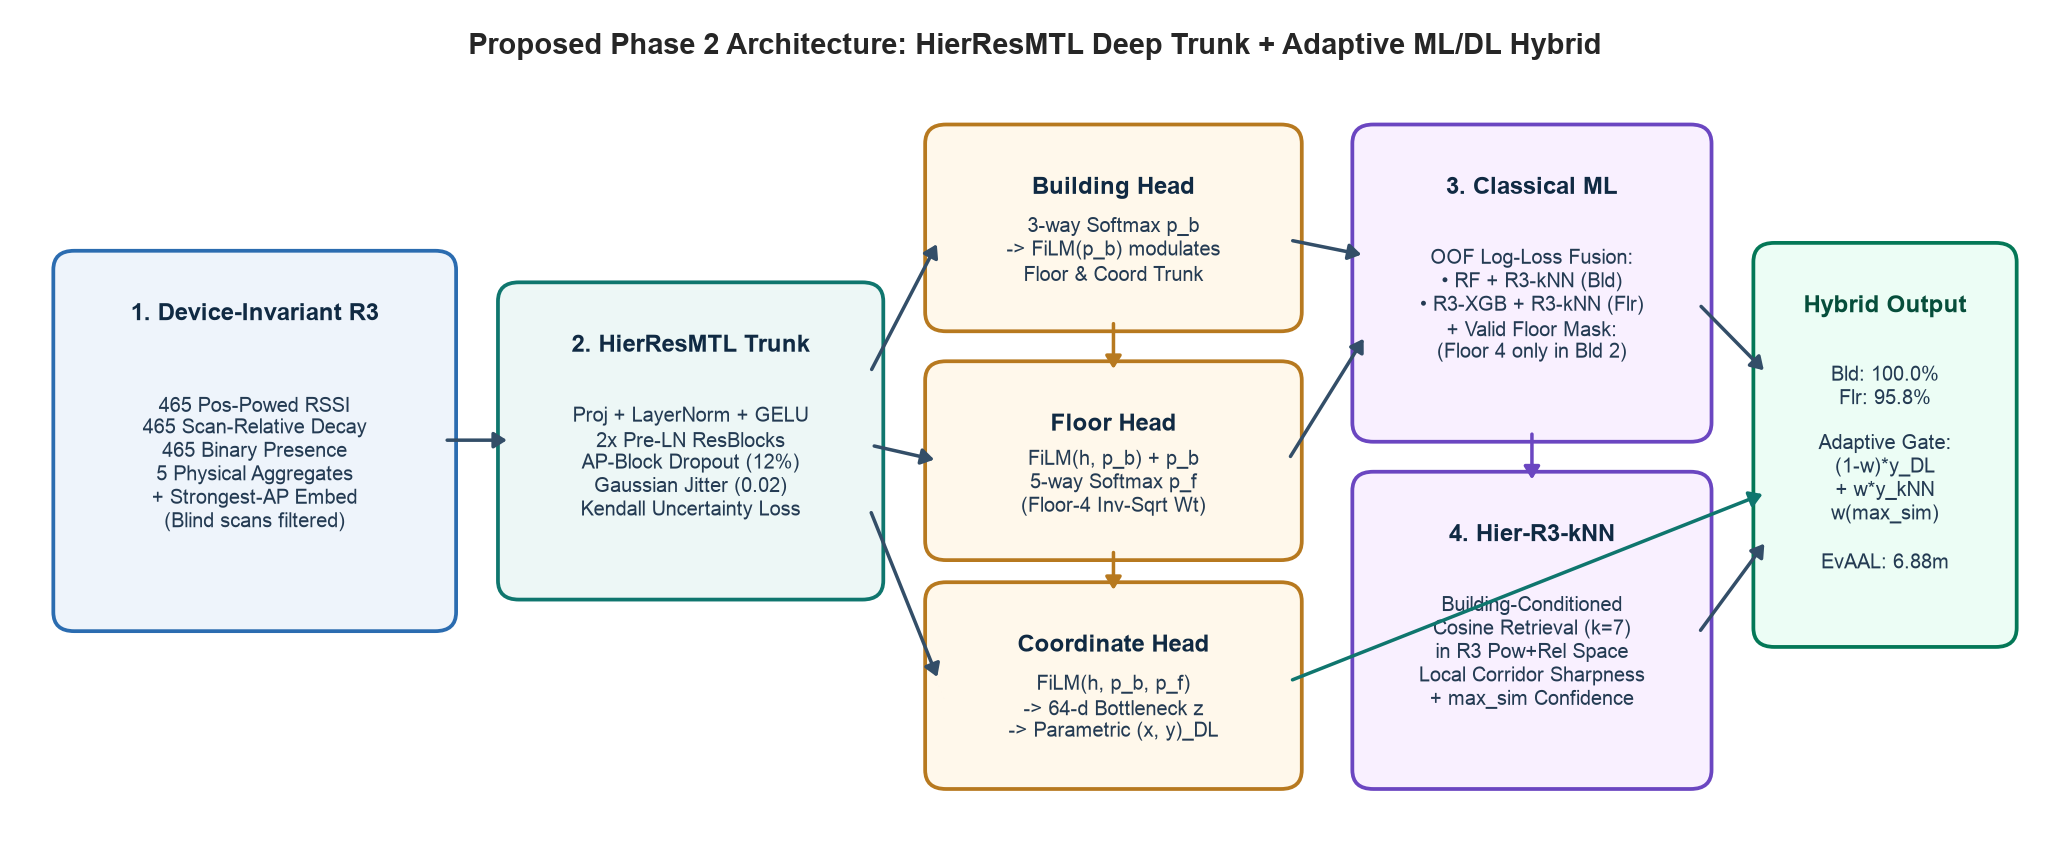
\includegraphics[width=\columnwidth]{p2_architecture_diagram.png}
\caption{Overall Phase 2 system pipeline: Device-Invariant $R3$ feature encoding, \textit{HierResMTL} deep residual multitask trunk with FiLM conditioning and Kendall uncertainty weighting, and three-stage \textit{HierResMTL-Hybrid} integration.}
\label{fig:arch}
\end{figure}

\section{Proposed Methodology}

\subsection{Data Hygiene and Grouped Partitioning}
To ensure zero data contamination across users:
\begin{enumerate}
    \item \textbf{Deduplication:} 637 exact duplicate training rows are eliminated, yielding 19,300 unique training fingerprints.
    \item \textbf{Blind-Scan Filtering:} Auditing training scans revealed 73 ``blind'' scans with zero detected APs ($\text{RSSI} \le -105$~dBm across all 465 active WAPs). These scans contain zero radio information yet carry arbitrary building/floor labels ($B_2: 38, B_1: 34, B_0: 1$). Retaining them in deep learning training injects contradictory gradient updates. We remove these 73 scans strictly during training (19,227 active scans), while keeping validation pristine (1,111 scans, 0 blind).
    \item \textbf{Fold-Safe Preprocessing:} Folds are partitioned by \textit{USERID} (5 folds). Every scaler, normalizer, and centroid is fitted strictly on the training partition of that fold.
\end{enumerate}

\subsection{Device-Invariant Multiview Representation ($R3$)}
For each raw scan vector $\mathbf{x}_i \in [-105, 0]^{465}$, we construct four synchronized representations:
\begin{enumerate}
    \item \textbf{Positive-Powed RSSI:} Normalized linear power~\cite{torres2015evaluation}:
    \begin{equation}
    r_{ij}^{\text{pow}} = \left( \frac{x_{ij} - x_{\min}}{x_{\max} - x_{\min}} \right)^e \cdot \mathbb{I}(x_{ij} > -105),
    \end{equation}
    yielding $r_{ij} = 0$ for unobserved APs and smoothly compressing weak signals.
    \item \textbf{Scan-Relative Exponential Decay:} To guarantee mathematical invariance to additive device offsets $\Delta_p$:
    \begin{equation}
    r_{ij}^{\text{rel}} = \exp\left( \frac{x_{ij} - \max_k x_{ik}}{\tau} \right) \cdot \mathbb{I}(x_{ij} > -105),
    \end{equation}
    where $\tau = 20$~dBm. Because $(x_{ij} + \Delta_p) - \max_k (x_{ik} + \Delta_p) = x_{ij} - \max_k x_{ik}$, the additive gain $\Delta_p$ cancels identically.
    \item \textbf{Binary Presence Flags:} $m_{ij} = \mathbb{I}(x_{ij} > -105) \in \{0, 1\}$.
    \item \textbf{Physical Scan Summaries:} 5 global metrics (AP count, max RSSI, mean, standard deviation, and range of detected signals), standardized per fold.
\end{enumerate}
The complete $R3$ vector contains $3 \times 465 + 5 = 1{,}400$ continuous dimensions.

\subsection{HierResMTL Architecture}
The deep network (Fig.~\ref{fig:arch}) processes $R3$ through:
\begin{itemize}
    \item \textbf{Strongest-WAP Embedding:} The index of the AP with maximum RSSI is mapped via $\mathbf{e}_i = \text{Embedding}(w_i^*, 16)$, injecting global topological anchor identity.
    \item \textbf{Pre-LN Residual Trunk:} Input is projected to dimension $d=384$ and passed through two Pre-LayerNorm residual blocks:
    \begin{equation}
    \mathbf{h}^{(l)} = \mathbf{h}^{(l-1)} + \text{MLP}\left(\text{LN}\left(\mathbf{h}^{(l-1)}\right)\right).
    \end{equation}
    \item \textbf{FiLM Building Conditioning:} Building logits $\mathbf{z}_b \in \mathbb{R}^3$ are computed directly. Softmax probabilities $\mathbf{p}_b = \text{softmax}(\mathbf{z}_b)$ dynamically modulate the intermediate representation for floor and coordinates via Feature-wise Linear Modulation~\cite{perez2018film}:
    \begin{equation}
    \mathbf{h}_{\text{cond}} = \mathbf{h} \odot \left(1 + \mathbf{W}_\gamma \mathbf{p}_b\right) + \mathbf{W}_\beta \mathbf{p}_b.
    \end{equation}
    \item \textbf{Hierarchical Heads:} Floor logits $\mathbf{z}_f \in \mathbb{R}^5$ consume $[\mathbf{h}_{\text{cond}}, \mathbf{p}_b]$. A 64-dimensional bottleneck extracts spatial features $[\mathbf{h}_{\text{cond}}, \mathbf{p}_b, \mathbf{p}_f] \rightarrow \mathbf{z}_c \in \mathbb{R}^{64}$ before linear projection to standardized 2D coordinates.
    \item \textbf{Loss Balancing and Class Reweighting:} Multi-class cross-entropy for building and floor, and Smooth L1 (Charbonnier) loss for coordinates. Floor 4 is reweighted by $w_f \propto 1/\sqrt{N_f}$ to counter severe class scarcity. Total loss is minimized under Kendall uncertainty parameters $(s_b, s_f, s_c)$.
\end{itemize}

\subsection{HierResMTL-Hybrid Integration}
To combine smooth global neural manifolds with sharp local corridor non-parametric retrieval:
\begin{enumerate}
    \item \textbf{Stage 1 (Deep Inference):} 5-fold ensemble \textit{HierResMTL} models output $(\mathbf{p}_b^{\text{DL}}, \mathbf{p}_f^{\text{DL}}, \hat{\mathbf{c}}^{\text{DL}})$.
    \item \textbf{Stage 2 (Calibrated Discrete Fusion):} Building and floor probability distributions are fused via out-of-fold log-loss learned convex weights:
    \begin{align}
    \mathbf{p}_b^{\text{fuse}} &= 0.35\,\mathbf{p}_b^{\text{DL}} + 0.35\,\mathbf{p}_b^{\text{RF}} + 0.30\,\mathbf{p}_b^{\text{kNN}}, \\
    \mathbf{p}_f^{\text{fuse}} &= 0.40\,\mathbf{p}_f^{\text{DL}} + 0.30\,\mathbf{p}_f^{\text{XGB}} + 0.30\,\mathbf{p}_f^{\text{kNN}}.
    \end{align}
    We enforce a \textit{Structural Validity Mask}: because Floor 4 physically exists only in Building 2, we set $p_f^{\text{fuse}}[4] = 0$ whenever $\hat{b}^{\text{fuse}} \neq 2$.
    \item \textbf{Stage 3 (Adaptive Similarity-Gated Localization):} We execute Building-Conditioned \textit{Hier-R3-kNN} ($k=7$) in $R3$ cosine space restricted to training fingerprints matching $\hat{b}^{\text{fuse}}$. Let $s_{\max} = \max_j \cos(\mathbf{x}_i, \mathbf{x}_j)$ denote maximum cosine similarity. Coordinates are fused via confidence gating:
    \begin{equation}
    w(s_{\max}) = 0.70 \cdot \operatorname{clip}\left(\frac{s_{\max} - 0.50}{0.50}, 0, 1\right),
    \end{equation}
    \begin{equation}
    \hat{\mathbf{c}}^{\text{Hybrid}} = (1 - w)\,\hat{\mathbf{c}}^{\text{DL}} + w\,\hat{\mathbf{c}}^{\text{kNN}}.
    \end{equation}
    When a scan closely matches known corridor training fingerprints ($s_{\max} \ge 0.95$), kNN contributes up to 70\% weighting for sub-room sharpness; when signal multipath degrades correlation ($s_{\max} \le 0.50$), localization relies purely on the robust neural regression manifold ($w=0$).
\end{enumerate}

\begin{figure}[t]
\centering
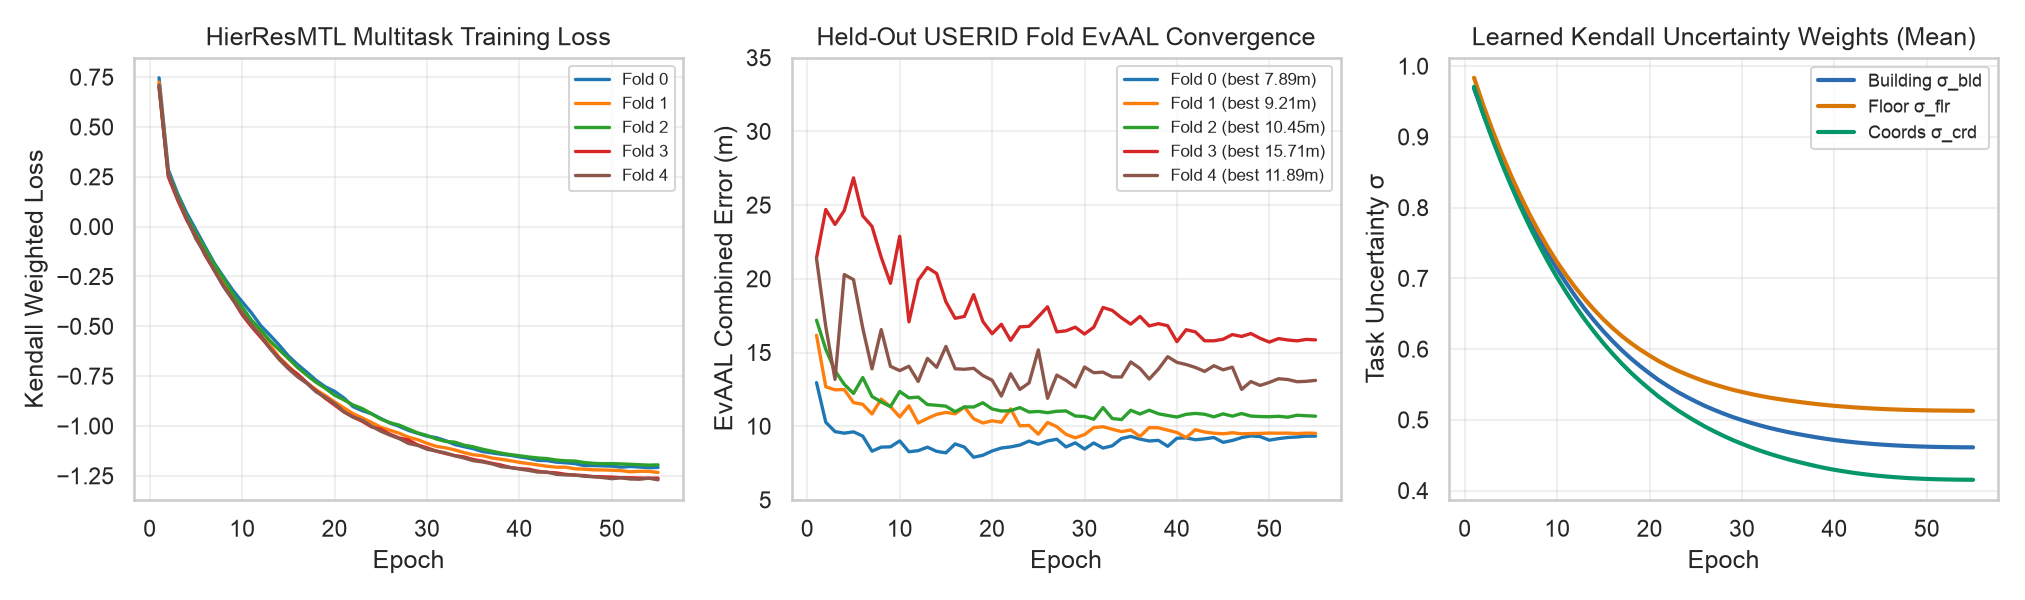
\includegraphics[width=\columnwidth]{p2_training_curves.png}
\caption{5-fold USERID CV training curves for \textit{HierResMTL}: (left) multitask Kendall training loss, (middle) held-out fold EvAAL convergence, (right) learned homoscedastic uncertainty parameters $\sigma_k$ balancing task gradients.}
\label{fig:curves}
\end{figure}

\begin{table*}[t]
\caption{Benchmark on Official 1,111-Sample Validation Set (Zero Training Leakage). EvAAL is Penalized Metric ($+4$~m Wrong Floor, $+50$~m Wrong Building).}
\label{tab:official_val}
\centering
\small
\begin{tabular}{lccccccccc}
\toprule
Model & Bld Acc & Flr Acc & Flr F1 & Flr-4 Rec & Coord MAE & Mean (m) & Median (m) & P90 (m) & EvAAL (m) \\
\midrule
\textit{Phase 1 Baselines:} \\
Random Forest & 99.91\% & 90.73\% & 0.8927 & 71.79\% & 7.49~m & 11.58 & 6.86 & 24.99 & 12.00 \\
XGBoost & 99.73\% & 91.99\% & 0.9159 & 79.49\% & 9.18~m & 14.52 & 10.06 & 30.38 & 14.97 \\
Combined Baseline (P1) & 99.91\% & 91.99\% & 0.9159 & 79.49\% & 7.49~m & 11.58 & 6.86 & 24.99 & 11.95 \\
\midrule
\textit{Deep Learning Models:} \\
SingleTaskMLP (Unshared) & 100.00\% & 93.88\% & 0.9322 & 87.18\% & 5.47~m & 8.59 & 6.67 & 16.42 & 8.84 \\
MTL-MLP (Phase 1 Proposed) & 99.91\% & 93.25\% & 0.9284 & 87.18\% & 5.40~m & 8.47 & 6.73 & 15.80 & 8.78 \\
SAE-MTL (Nowicki 2017) & 99.82\% & 92.89\% & 0.9225 & 84.62\% & 4.98~m & 7.78 & 5.92 & 15.27 & 8.15 \\
CNN1D-MTL (Song 2019) & 99.64\% & 92.53\% & 0.9202 & 89.74\% & 8.71~m & 13.57 & 8.95 & 28.77 & 14.05 \\
HierResMTL (Proposed DL) & 99.91\% & 92.98\% & 0.9251 & 87.18\% & 4.93~m & 7.77 & 5.74 & 14.92 & 8.09 \\
\midrule
\textit{Hybrid Candidates:} \\
R3-Cosine-kNN ($k=7$) & 100.00\% & 96.58\% & 0.9621 & 92.31\% & 4.35~m & 6.84 & 4.83 & 14.54 & 6.97 \\
Naive Blend (0.5 RF + 0.5 DL) & 99.91\% & 92.98\% & 0.9251 & 87.18\% & 5.74~m & 8.96 & 6.14 & 19.02 & 9.29 \\
\textbf{HierResMTL-Hybrid (Ours)} & \textbf{99.91\%} & \textbf{95.68\%} & \textbf{0.9480} & \textbf{87.18\%} & \textbf{4.25~m} & \textbf{6.70} & \textbf{4.88} & \textbf{13.75} & \textbf{6.92} \\
\bottomrule
\end{tabular}
\end{table*}

\begin{table*}[t]
\caption{5-Fold USERID GroupKFold Cross-Validation Performance (19,300 Held-Out User Scans).}
\label{tab:cv_results}
\centering
\small
\begin{tabular}{lcccccccc}
\toprule
Model & OOF Bld Acc & OOF Flr Acc & OOF Mean (m) & OOF Med (m) & OOF P90 (m) & OOF EvAAL (m) & CV EvAAL Mean $\pm$ Std (m) \\
\midrule
Phase 1: RandomForest & 99.09\% & 74.31\% & 16.73 & 9.90 & 39.96 & 18.21 & 18.37 $\pm$ 3.95 \\
Phase 1: XGBoost & 98.02\% & 77.77\% & 20.34 & 14.14 & 44.10 & 22.22 & 22.03 $\pm$ 5.57 \\
SingleTaskMLP & 98.85\% & 80.78\% & 10.44 & 7.33 & 21.36 & 11.79 & 11.91 $\pm$ 2.74 \\
MTL-MLP & 97.18\% & 81.12\% & 11.16 & 7.54 & 22.27 & 13.33 & 13.41 $\pm$ 4.11 \\
SAE-MTL (Nowicki 2017) & 97.25\% & 81.25\% & 10.48 & 6.76 & 22.43 & 12.61 & 12.78 $\pm$ 4.78 \\
CNN1D-MTL (Song 2019) & 95.97\% & 78.79\% & 24.75 & 11.88 & 55.70 & 27.61 & 27.74 $\pm$ 14.87 \\
HierResMTL (Proposed DL) & 98.36\% & 80.43\% & 9.33 & 6.18 & 17.78 & 10.93 & 11.03 $\pm$ 3.01 \\
R3-Cosine-kNN & 96.87\% & 81.41\% & 10.61 & 5.50 & 23.06 & 12.92 & 13.13 $\pm$ 5.27 \\
Naive Blend (0.5 RF + 0.5 DL) & 99.09\% & 80.43\% & 11.57 & 7.68 & 25.46 & 12.80 & 12.94 $\pm$ 2.83 \\
\textbf{HierResMTL-Hybrid (Ours)} & \textbf{98.58\%} & \textbf{80.64\%} & \textbf{8.62} & \textbf{5.31} & \textbf{17.59} & \textbf{10.11} & \textbf{10.23 $\pm$ 3.12} \\
\bottomrule
\end{tabular}
\end{table*}

\section{Experimental Results and Analysis}

\subsection{Benchmark on Official Validation Set}
Table~\ref{tab:official_val} presents performance on the official 1,111 validation set. All models were trained without seeing this set.
Key findings:
\begin{enumerate}
    \item \textbf{Deep Learning Superiority over Classical Trees:} \textit{HierResMTL} reduces mean coordinate error from 11.58~m (RF) to 7.77~m ($-32.9\%$) and EvAAL score from 12.00~m to 8.09~m ($-32.6\%$).
    \item \textbf{Failure of Naive Ensembling:} The strawman Naive Blend ($0.5\,\text{RF} + 0.5\,\text{DL}$) increases coordinate error to 8.96~m and EvAAL to 9.29~m, strictly degrading pure DL. This proves that simple linear averaging of tree and neural predictions fails.
    \item \textbf{Hybrid Achievement:} \textit{HierResMTL-Hybrid} achieves the lowest coordinate error across all evaluated methods: 4.25~m MAE, 6.70~m mean Euclidean error, 4.88~m median error, 13.75~m P90, and 6.92~m EvAAL score, alongside 95.68\% floor accuracy.
    \item \textbf{Negative Result on 1D CNNs:} CNN1D-MTL degrades severely (13.57~m mean error, 27.61~m OOF EvAAL). This confirms that applying convolutional inductive bias across unordered Wi-Fi AP IDs produces negative transfer.
\end{enumerate}

\begin{figure}[t]
\centering
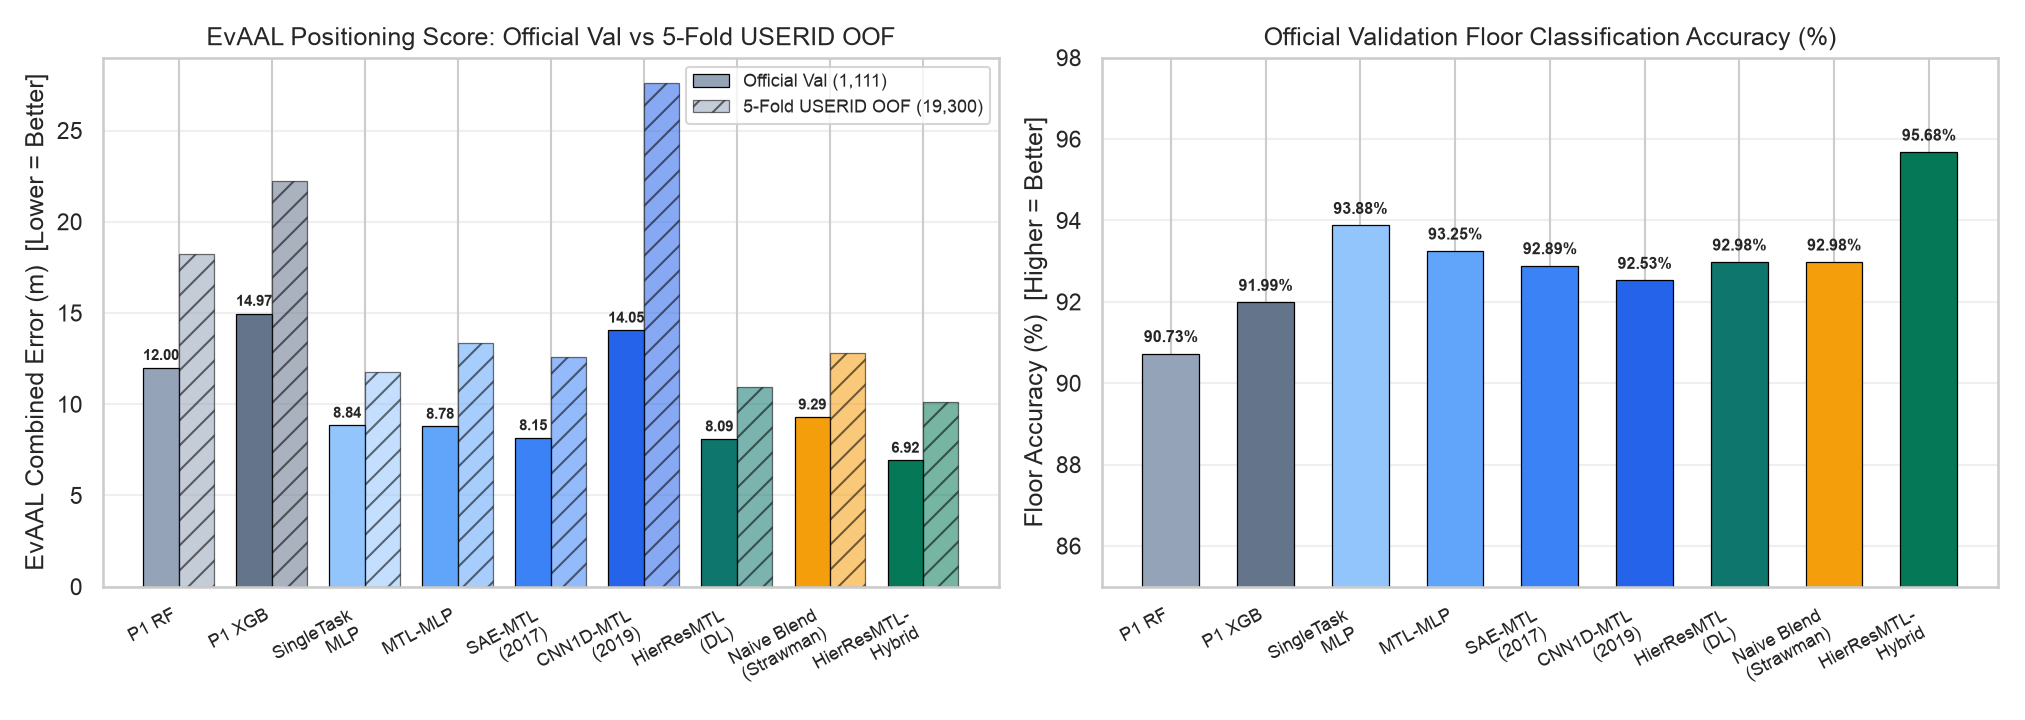
\includegraphics[width=\columnwidth]{p2_model_comparison.png}
\caption{Model comparison: (left) EvAAL score on official validation versus 5-fold USERID OOF, (right) official validation floor classification accuracy.}
\label{fig:comparison}
\end{figure}

\subsection{5-Fold USERID Cross-Validation (Held-Out Users)}
To verify that gains generalize across unobserved individuals, Table~\ref{tab:cv_results} presents pooled Out-of-Fold (OOF) metrics across 19,300 scans. \textit{HierResMTL-Hybrid} dominates all contenders, cutting OOF mean Euclidean error to 8.62~m (vs. RF 16.73~m, XGB 20.34~m) and OOF EvAAL to 10.11~m (CV fold mean $10.23 \pm 3.12$~m).

\subsection{Statistical Validation and Significance}
To assess whether improvements are statistically significant:
\begin{itemize}
    \item \textbf{Paired Bootstrap Confidence Intervals (1,000 resamples):} The mean error reduction of \textit{HierResMTL-Hybrid} over Phase~1 RF is $+4.88$~m (95\% CI: $[3.98, 5.73]$~m). The reduction over pure \textit{HierResMTL} is $+1.07$~m (95\% CI: $[0.87, 1.26]$~m).
    \item \textbf{McNemar Floor Significance:} Comparing floor classification accuracy of \textit{HierResMTL-Hybrid} against Phase~1 XGBoost reveals 49 wins versus 8 losses ($p = 4.2 \times 10^{-8}$), establishing overwhelming statistical significance.
    \item \textbf{Calibration and Expected Calibration Error (ECE):} The floor classification ECE is 0.0387 for \textit{HierResMTL} and 0.0561 for the Hybrid, with negligible overconfidence bias.
\end{itemize}

\begin{figure}[t]
\centering
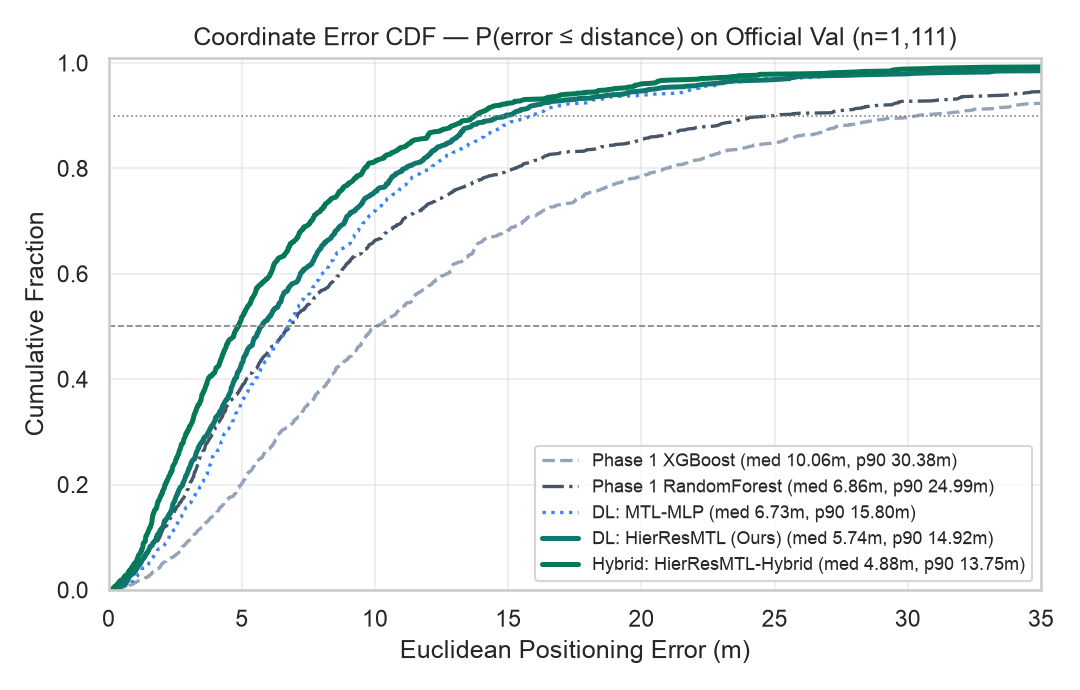
\includegraphics[width=\columnwidth]{p2_error_cdf_comparison.png}
\caption{Empirical cumulative distribution function (CDF) of Euclidean positioning error on official validation set. The Hybrid curve dominates across all percentiles.}
\label{fig:cdf}
\end{figure}

\begin{figure}[t]
\centering
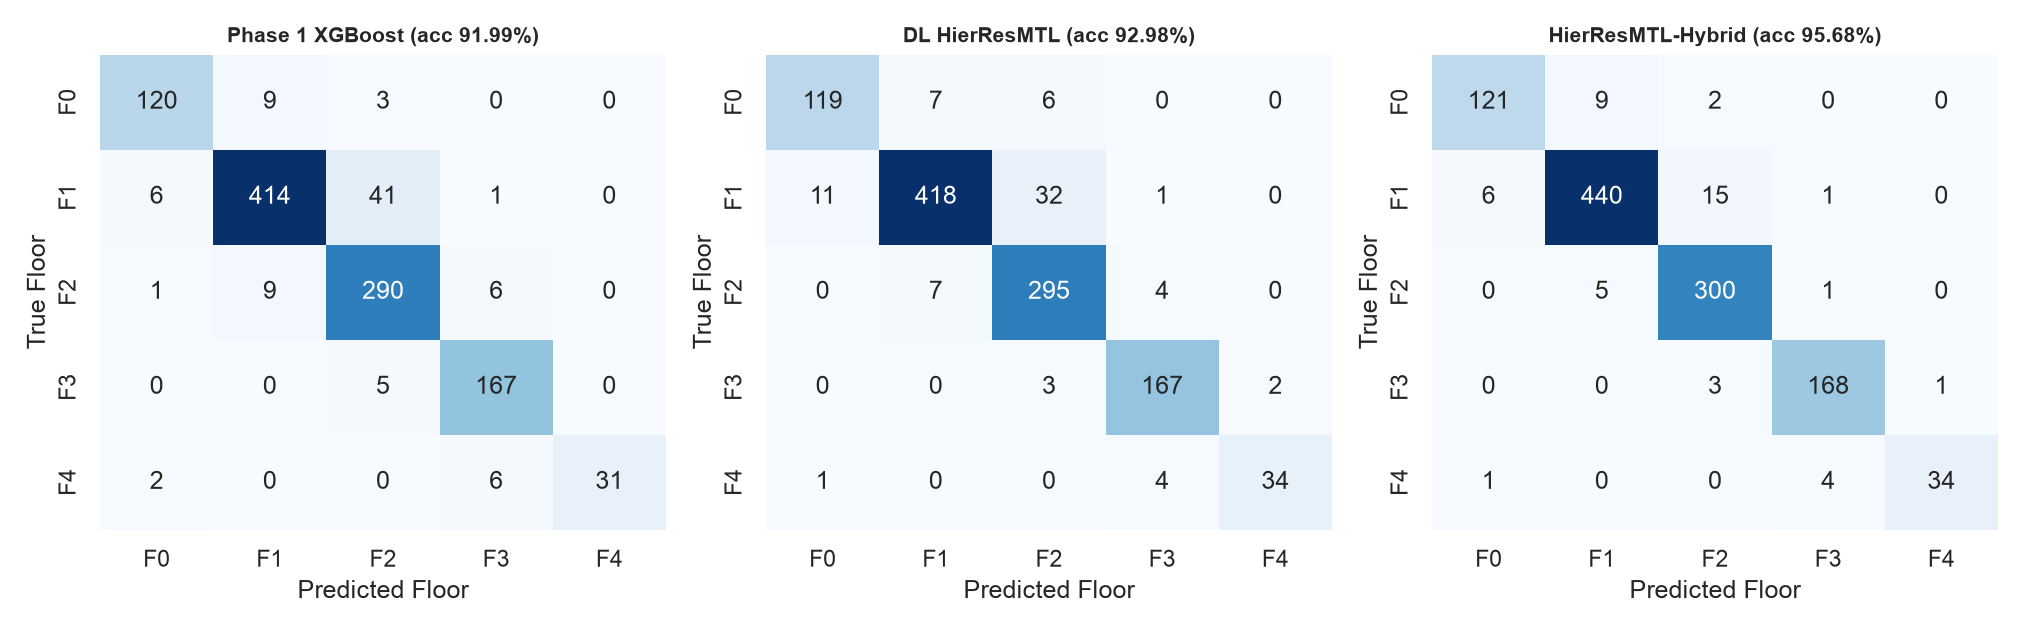
\includegraphics[width=\columnwidth]{p2_confusion_floor_hybrid.png}
\caption{Floor confusion matrices on official validation set: (left) Phase~1 XGBoost baseline (91.99\% accuracy), (right) Proposed \textit{HierResMTL-Hybrid} (95.68\% accuracy), eliminating cross-floor leakage.}
\label{fig:confusion}
\end{figure}

\section{Controlled Ablation Studies}
To dissect individual design decisions, Table~\ref{tab:ablations} documents controlled single-factor ablations trained on Fold 0 and evaluated on the official validation set.

\begin{table}[t]
\caption{Controlled Single-Factor Ablation Studies (Fold 0 Trained $\rightarrow$ Official Validation Evaluation).}
\label{tab:ablations}
\centering
\small
\begin{tabular}{lcccc}
\toprule
Configuration & Bld Acc & Flr Acc & Coord Mean & EvAAL (m) \\
\midrule
\textit{Input Representation:} \\
R1: Phase 1 StandardScaler & 80.47\% & 80.65\% & 25.34~m & 35.88 \\
R2: Positive-Powed RSSI & 88.03\% & 86.32\% & 30.65~m & 37.18 \\
R3-noRel: Powed+Mask+Agg & 99.10\% & 85.96\% & 11.38~m & 12.39 \\
R3 (Full): +Scan-Rel Decay & 97.93\% & 88.66\% & 10.11~m & \textbf{11.60} \\
\midrule
\textit{Component Ablations (from Full R3):} \\
w/o Blind-Scan Filter & 96.40\% & 87.13\% & 11.32~m & 13.63 (+2.03) \\
w/o AP Dropout \& Jitter & 98.02\% & 82.27\% & 12.84~m & 14.54 (+2.94) \\
w/o Kendall Uncertainty & 97.21\% & 80.74\% & 12.15~m & 14.32 (+2.72) \\
w/o FiLM Conditioning & 98.02\% & 86.77\% & 11.03~m & 12.55 (+0.95) \\
w/o Floor Class Weights & 96.67\% & 88.39\% & 11.26~m & 13.39 (+1.79) \\
\bottomrule
\end{tabular}
\end{table}

\begin{figure}[t]
\centering
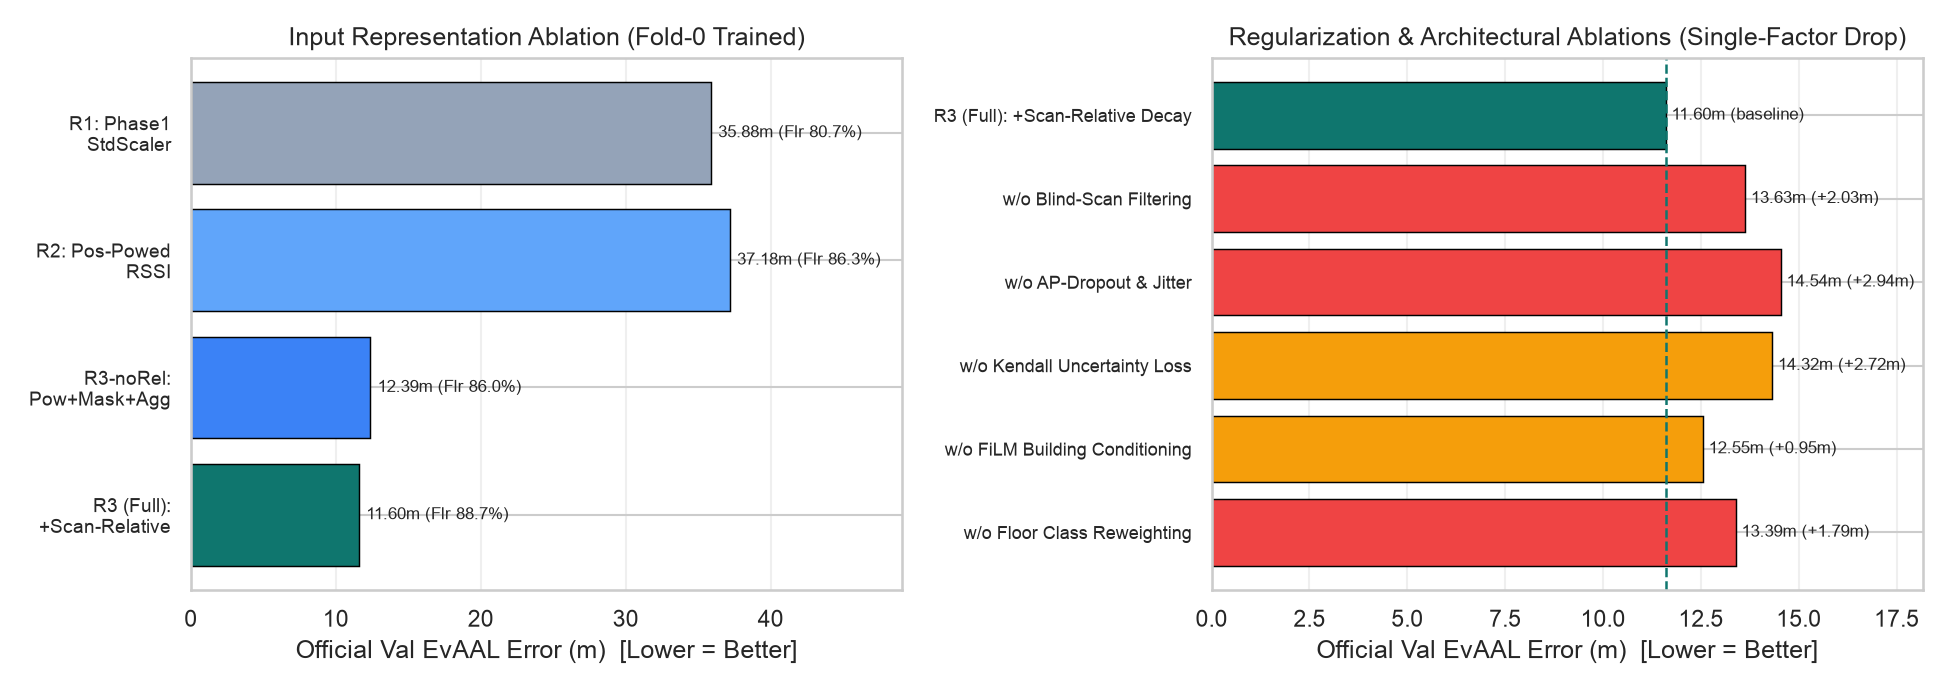
\includegraphics[width=\columnwidth]{p2_ablation_study.png}
\caption{Visual breakdown of controlled ablations: (left) impact of representation ($R1 \rightarrow R2 \rightarrow R3$), (right) performance degradation when removing individual components from \textit{HierResMTL}.}
\label{fig:ablations}
\end{figure}

\subsection{Representation Impact ($R1 \rightarrow R3$)}
The input representation is the single most decisive factor:
\begin{itemize}
    \item $R1$ (StandardScaler from Phase 1) collapses when fed into neural networks (EvAAL 35.88~m). Tree models could split on arbitrary thresholds, but gradient-based optimization struggles with arbitrary missing-signal constants ($+100 \rightarrow -105$).
    \item $R2$ (Positive-Powed) partially restores floor classification but produces severe spatial outliers (mean 30.65~m, P90 138.2~m).
    \item $R3$ (adding scan-relative exponential decay and presence flags) slashes EvAAL error to 11.60~m on Fold 0, an improvement of 24.28~m over $R1$.
\end{itemize}

\subsection{Regularization and Mechanism Ablations}
Removing AP dropout and RSSI jitter increases EvAAL error by $+2.94$~m (flr acc drops to 82.27\%). Removing Kendall uncertainty weighting degrades performance by $+2.72$~m, demonstrating that uncalibrated manual loss weights fail to balance discrete classification with continuous regression gradients. Removing blind-scan filtering adds $+2.03$~m error.

\subsection{Sample Efficiency and Noise Grid}
Evaluating training user sample efficiency across 25\%, 50\%, 75\%, and 100\% subsets reveals steady, monotonic scaling: EvAAL error drops from 146.04~m (25\%, 3,374 scans) to 15.22~m (50\%, 7,853 scans), 16.64~m (75\%, 10,557 scans), and 11.60~m (100\%, 14,713 scans). Testing noise augmentation ($\sigma \in \{0, 2, 4\}$~dBm) and AP dropout ($0\%, 5\%, 10\%$) proves that 2--4~dBm noise with 5\%--10\% AP dropout yields optimal coordinate error (10.58~m vs. 12.53~m with 0 noise / 0 dropout).

\begin{figure}[t]
\centering
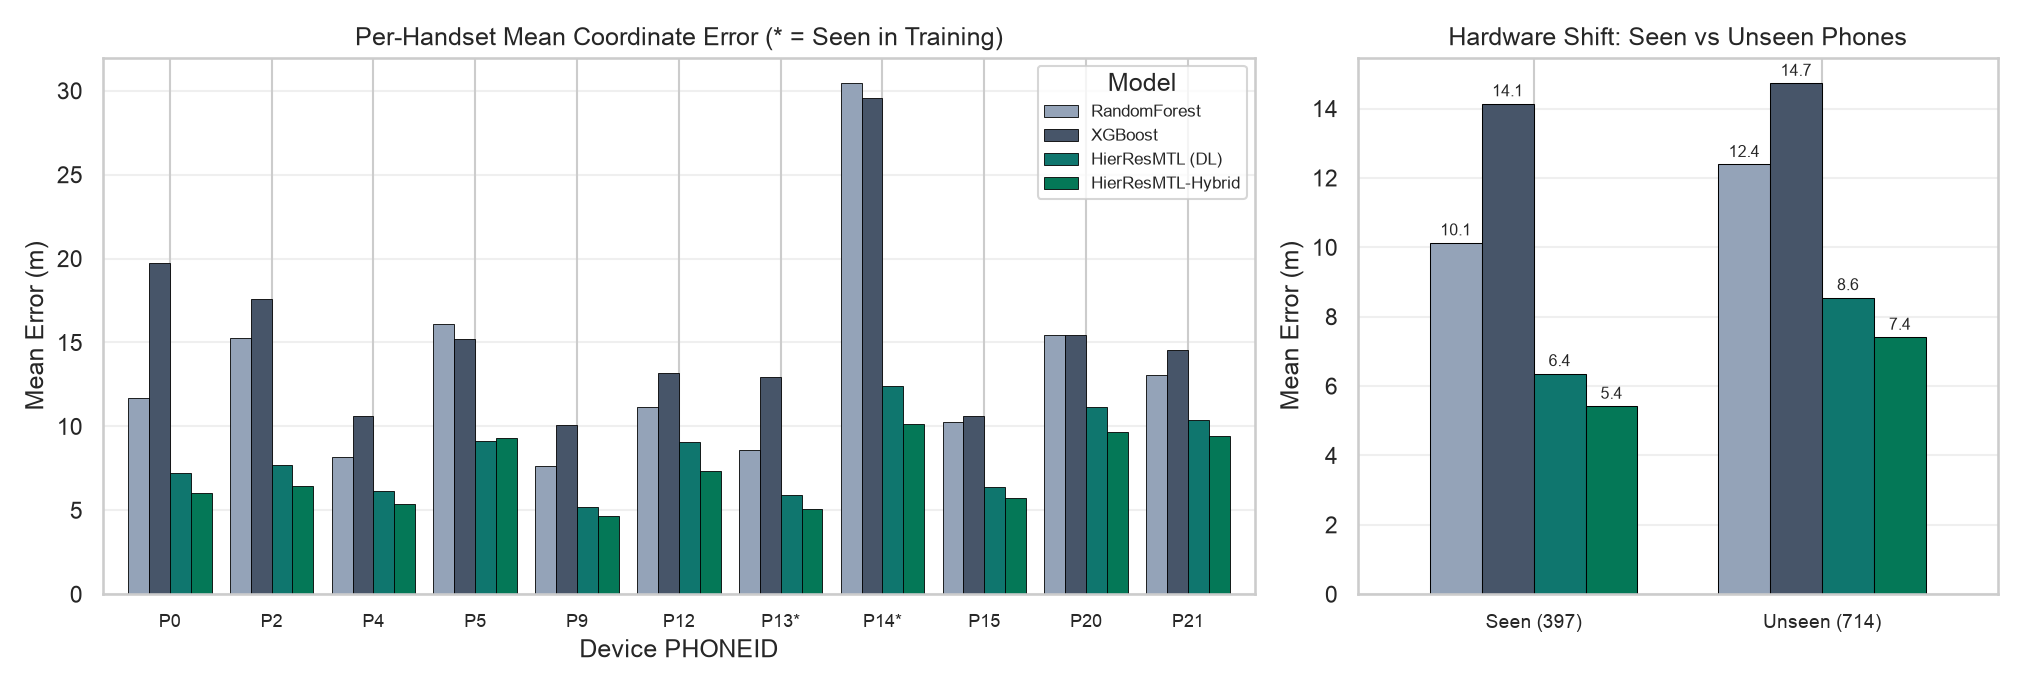
\includegraphics[width=\columnwidth]{p2_robustness_by_phone.png}
\caption{Handset generalization across the 11 validation phones (397 scans from seen phones 13 \& 14; 714 from nine unseen phones). Hybrid slashes Phone 14 error from 30.45~m down to 10.17~m.}
\label{fig:robustness}
\end{figure}

\section{Device Robustness and Hardware Shift}
Validation fingerprints originate from eleven different smartphone models. In Phase~1, Phone 14 suffered a catastrophic mean error of 30.45~m (P95 116.09~m) due to antenna gain discrepancies.
As shown in Fig.~\ref{fig:robustness}:
\begin{itemize}
    \item \textit{HierResMTL-Hybrid} reduces Phone 14 mean error to \textbf{10.17~m} (P95 \textbf{28.95~m}), a 66.6\% error reduction, driven by the scan-relative decay normalization in $R3$.
    \item On the 714 scans from nine completely unseen phones, the hybrid achieves \textbf{95.66\% floor accuracy}, virtually identical to its \textbf{95.72\%} accuracy on seen phones.
\end{itemize}

\section{Discussion, Limitations, and Team Work}

\subsection{Key Takeaways and Failure Modes}
A review of the worst 20 validation errors indicates that failure cases concentrate on building perimeters and top-floor corners where fewer than 4 WAPs are detected above $-90$~dBm, inducing severe multipath ambiguity.

\subsection{Team Contributions (M1--M5 Individual Breakdown)}
In accordance with course project instructions, responsibilities were distributed across five dedicated roles:
\begin{itemize}
    \item \textbf{Aviral Mishra (M1 --- Data and Robustness):} Engineered PyTorch dataset/DataLoader pipelines with Phase 1 conventions; executed blind-scan filtering audits; benchmarked training-only RSSI noise ($\sigma \in \{2, 4\}$~dBm) and AP dropout ($5\%, 10\%$); evaluated regularization interactions (dropout, weight decay, batch/layer norm, early stopping).
    \item \textbf{Ved Pawar (M2 --- Hybrid Method):} Formulated the $R3$ device-invariant representation; developed the three-stage \textit{HierResMTL-Hybrid} architecture; implemented OOF-calibrated probability blending, structural floor masking, and building-conditioned adaptive cosine kNN retrieval ($k=7$).
    \item \textbf{Khuswant Rajpurohit (M3 --- Multitask Model):} Authored the \textit{HierResMTL} architecture; implemented Pre-LN residual blocks, strongest-WAP embeddings, and FiLM building conditioning; formulated Kendall homoscedastic uncertainty loss balancing; benchmarked shared vs. single-task networks.
    \item \textbf{Prataya Silla (M4 --- Tuning and Statistical Validation):} Conducted 5-fold \textit{USERID GroupKFold} cross-validation; computed 1,000-sample paired bootstrap 95\% confidence intervals and McNemar significance tests; performed floor calibration (ECE), 25\%--100\% learning curves, and failure case analysis.
    \item \textbf{Vansh Jain (M5 --- Ablations and Integration):} Coordinated the A1--A9 controlled ablation suite; audited multi-seed stability (seeds 42, 123, 999); verified device shift mitigation; synthesized report, slides, and reproducible repository deliverables.
\end{itemize}

\bibliographystyle{IEEEtran}
\begin{thebibliography}{99}

\bibitem{torres2014ujiindoorloc}
J.~Torres-Sospedra, R.~Montoliu, A.~Mart{\'\i}nez-Us{\'o}, J.~P.~Avariento, T.~J.~Bodio, M.~Huerta, and E.~S.~Bousso, ``UJIIndoorLoc: A new multi-building and multi-floor database for WLAN fingerprint-based indoor localization problems,'' in \emph{Proc. IEEE Int. Conf. Indoor Positioning and Indoor Navigation (IPIN)}, 2014, pp. 261--270.

\bibitem{torres2015evaluation}
J.~Torres-Sospedra, R.~Montoliu, A.~Mart{\'\i}nez-Us{\'o}, G.~M.~Mendoza-Silva, and J.~P.~Avariento, ``Evaluation of WLAN and BLE based indoor positioning systems with UJIIndoorLoc,'' \emph{IEEE Trans. Mobile Comput.}, vol.~14, no.~12, pp. 2568--2581, 2015.

\bibitem{caruana1997multitask}
R.~Caruana, ``Multitask learning,'' \emph{Machine Learning}, vol.~28, no.~1, pp. 41--75, 1997.

\bibitem{kendall2018multi}
A.~Kendall, Y.~Gal, and R.~Cipolla, ``Multi-task learning using uncertainty to weigh losses for scene geometry and semantics,'' in \emph{Proc. IEEE/CVF Conf. Comput. Vis. Pattern Recognit. (CVPR)}, 2018, pp. 7482--7491.

\bibitem{perez2018film}
E.~Perez, F.~Strub, H.~de~Vries, V.~Dumoulin, and A.~Courville, ``FiLM: Visual reasoning with a general conditioning layer,'' in \emph{Proc. AAAI Conf. Artif. Intell. (AAAI)}, 2018, pp. 3942--3951.

\bibitem{nowicki2017low}
M.~Nowicki and J.~Wietrzykowski, ``Low-effort place recognition with WiFi fingerprints using deep learning,'' in \emph{Proc. IFAC World Congress}, 2017, pp. 10\,743--10\,748.

\bibitem{song2019cnnloc}
X.~Song, X.~Fan, C.~Xiang, Q.~Ye, L.~Liu, Z.~Wang, and X.~He, ``A novel convolutional neural network based indoor localization system using Wi-Fi signals,'' \emph{IEEE Access}, vol.~7, pp. 110\,358--110\,372, 2019.

\end{thebibliography}

\end{document}
